

\[
e \quad IC(\mu) = \left( \bar{X}_n \pm z_{\alpha/2} \frac{\sigma}{\sqrt{n}} \right)_{1-\alpha}
\]

\textbf{Q (5.7)} Sejam $X_1, \ldots, X_n$ i.i.d. de $X \sim N(\mu, \sigma^2)$ com $\mu \in \mathbb{R}$ e $\sigma^2 > 0$ desconhecido. Encontre estimador bilateral intervalar com $1-\alpha$ de confiança para $\mu$.

\textbf{Solução:} \\
Dai de discussões anteriores $(\bar{X}_n, S)$ é uma estatística suficiente mínima para $(\mu, \sigma)$. Aqui, $X_i$'s têm família de locação-escala.

Note que
\begin{equation}
U = \sqrt{n} \frac{\bar{X}_n - \mu}{S_n} \sim t_{n-1} \quad \text{é um pivô}.
\end{equation}

Para $t_{n-1, \alpha/2} > 0$ tal que
\begin{equation}
P\left( U > t_{n-1, \alpha/2} \right) = \frac{\alpha}{2}
\end{equation}

\begin{center}
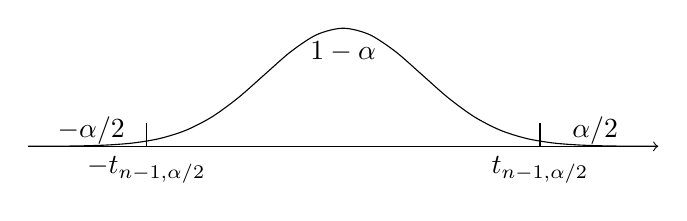
\begin{tikzpicture}
\draw[->] (-4,0) -- (4,0);
\draw[domain=-4:4,smooth,variable=\x] plot ({\x},{1.5*exp(-\x*\x/2)});
\draw (-2.5,0) -- (-2.5,0.3);
\draw (2.5,0) -- (2.5,0.3);
\node at (0,1.2) {$1-\alpha$};
\node at (-3.2,0.2) {$-\alpha/2$};
\node at (3.2,0.2) {$\alpha/2$};
\node at (-2.5,-0.3) {$-t_{n-1,\alpha/2}$};
\node at (2.5,-0.3) {$t_{n-1,\alpha/2}$};
\end{tikzpicture}
\end{center}

Tem-se
\begin{equation}
P\left\{ -t_{n-1,\alpha/2} < U < t_{n-1,\alpha/2} \right\} = 1 - \alpha
\end{equation}

\[
\therefore P\left\{ -t_{n-1,\alpha/2} < \sqrt{n} \frac{\bar{X}_n - \mu}{S_n} < t_{n-1,\alpha/2} \right\} = 1 - \alpha
\]

\[
\therefore P\left\{ \mu \in \left( \bar{X}_n \pm t_{n-1,\alpha/2} \frac{S_n}{\sqrt{n}} \right) \right\} = 1 - \alpha
\]

\[
IC(\mu) = \left[ \bar{X} \pm t_{n-1,\alpha/2} \frac{S_n}{\sqrt{n}} \right]_{(1-\alpha)}
\]
